\documentclass{article}
\PassOptionsToPackage{numbers,sort&compress}{natbib}
\usepackage[preprint]{neurips_2026}
\makeatletter
\renewcommand{\@noticestring}{}
\makeatother
\usepackage[utf8]{inputenc}
\usepackage[T1]{fontenc}
\usepackage{amsmath,amssymb}
\usepackage{booktabs,tabularx}
\usepackage{graphicx}
\usepackage{placeins}
\usepackage{xcolor}
\usepackage{tikz}
\usetikzlibrary{arrows.meta,positioning}
\usepackage{microtype}
\usepackage{url}
\usepackage[colorlinks=true,linkcolor=blue!50!black,citecolor=blue!50!black,urlcolor=blue!50!black]{hyperref}
\hypersetup{
  pdftitle={Motion Prediction through Physical Laws: State Estimation and Collision-Aware Simulation from Video},
  pdfauthor={Dong Wang},
  pdfsubject={An exploratory study of object-state estimation and two-dimensional motion prediction}
}

\title{Motion Prediction through Physical Laws:\\
State Estimation and Collision-Aware Simulation from Video}
\author{
  Dong Wang \\
  Purdue University \\
  \texttt{wang6213@purdue.edu}\\[3pt]
  \small\href{https://aabbccdkg.github.io/Video_prediction_through_physical_laws/}{Project page and synchronized video demos}
}

\newcommand{\pos}{\mathbf{p}}
\newcommand{\vel}{\mathbf{v}}
\newcommand{\acc}{\mathbf{a}}
\newcommand{\state}{\mathbf{s}}
\newcommand{\params}{\boldsymbol{\theta}}

\begin{document}
\maketitle

\begin{abstract}
Predicting object motion from video requires estimating a scene's state and representing the interactions that change it. In billiards scenes, trajectories are locally smooth between contacts, while collisions introduce abrupt changes in velocity. We present a framework that separates these two regimes through object-state estimation and rigid-body simulation. Circular-object detections provide position observations; local quadratic fits yield analytic estimates of velocity and acceleration; a two-dimensional physics engine advances the resulting states and resolves object contacts. The output is a sequence of predicted geometric configurations that can be rendered independently of object texture. A reference prototype combines OpenCV, SciPy, and Pymunk with screen recordings of Real Pool 3D. We formulate the state representation, time conventions, contact transitions, and evaluation criteria, and analyze the sensitivity of fitted dynamics to observation noise. An exploratory experiment uses twenty recordings grouped into training, validation, and evaluation scenes, with separately measured image trajectories and a compact ConvLSTM baseline trained across three random seeds. The comparisons isolate the effect of contacts using identical estimated states and distinguish geometric accuracy from full-frame reconstruction. The scope is limited to this small virtual-scene collection and its image-derived reference measurements.
\end{abstract}

\section{Introduction}

Video prediction combines visual inference with temporal reasoning. An observed frame provides evidence about object position and appearance, but generally does not determine velocity, acceleration, or future interactions. Recovering these quantities from a sequence allows a predictor to represent motion at the level of object states rather than relying exclusively on image-space continuation.

Billiards illustrates the distinction between smooth motion and discrete interaction events. Between contacts, a ball's trajectory admits a local parametric approximation. During a collision, its velocity changes abruptly. Continuing a pre-contact polynomial through that event can produce an incorrect trajectory even when the polynomial fits the observed positions closely. The difficulty is therefore not limited to extrapolating a smooth curve: it also includes predicting when contact occurs and how that contact changes the state.

We formulate a pipeline that combines local trajectory estimation with an explicit contact solver. Circle detection extracts object centers and radii from an observed video prefix. Trajectory fitting converts the centers into estimates of position, velocity, and acceleration at a common forecast origin. A rigid-body simulator then advances the scene and applies contact-dependent velocity updates. The resulting geometry is rendered as an outline sequence. Figure~\ref{fig:pipeline} shows the information flow.

\begin{figure}[t]
  \centering
  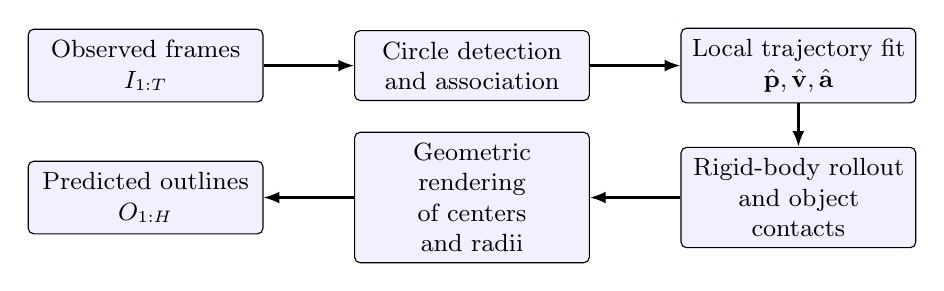
\begin{tikzpicture}[
  block/.style={draw,rounded corners=2pt,align=center,
                minimum height=0.85cm,text width=2.70cm,
                inner sep=4pt,font=\small},
  flow/.style={-{Latex[length=2mm]},thick},
  node distance=0.55cm and 1.15cm
]
  \node[block,fill=blue!6] (frames) {Observed frames\\$I_{1:T}$};
  \node[block,fill=blue!6,right=of frames] (detect) {Circle detection\\and association};
  \node[block,fill=blue!6,right=of detect] (fit) {Local trajectory fit\\$\hat\pos,\hat\vel,\hat\acc$};
  \node[block,fill=blue!6,below=of fit] (physics) {Rigid-body rollout\\and object contacts};
  \node[block,fill=blue!6,left=of physics] (render) {Geometric rendering\\of centers and radii};
  \node[block,fill=blue!6,left=of render] (outlines) {Predicted outlines\\$O_{1:H}$};
  \draw[flow] (frames) -- (detect);
  \draw[flow] (detect) -- (fit);
  \draw[flow] (fit) -- (physics);
  \draw[flow] (physics) -- (render);
  \draw[flow] (render) -- (outlines);
\end{tikzpicture}

  \caption{Object-state prediction framework. The observed prefix supplies position measurements for local trajectory fitting. The estimated state initializes a rigid-body rollout, whose object configurations determine the predicted outlines.}
  \label{fig:pipeline}
\end{figure}

This representation makes several modeling choices inspectable. Detection controls the quality of the observations; association determines which measurements belong to the same object; fitting determines the initial motion state; and the simulator specifies the response to contact. It also separates geometric prediction from texture synthesis, so that errors in motion can be examined independently of image appearance.

This report formulates an object-state framework for planar circular objects, local smooth-motion estimation, and contact transitions. A reference prototype combines classical detection with a conventional physics engine~\citep{projectrepo}. The study analyzes the framework's assumptions and reports grouped comparisons of smooth extrapolation, contact simulation, and a compact learned predictor on existing recordings. Its contribution is a reproducible restricted-domain comparison and contact ablation; it does not introduce object-centered physical prediction as a new general principle.

\section{Related work}

\paragraph{Image-space sequence prediction.}
ConvLSTM uses convolutional input-to-state and state-to-state transitions to represent spatiotemporal observations~\citep{shi2015convlstm}. Such models learn a mapping from an observed sequence to its continuation. An object-state representation instead exposes geometric variables and the transition rules acting on them. The two representations support different diagnostics: image reconstruction describes the predicted visual field, while tracked states permit direct measurement of displacement and contact behavior.

\paragraph{Object and interaction models.}
Interaction Networks represent objects and their relations to learn physical transitions~\citep{battaglia2016interaction}. Visual Interaction Networks connect observations from video to object-based dynamics prediction~\citep{watters2017visual}. These works motivate explicit relational structure in motion models. The framework considered here uses a classical detector for circular objects and a rigid-body solver for contacts, restricting the visual domain in exchange for directly interpretable state variables.

\paragraph{Physical dynamics and appearance.}
PhyDNet separates constrained physical dynamics from complementary factors in a learned video predictor~\citep{leguen2020phydnet}. The present framework separates them through explicit geometry: motion is represented by object centers and radii, and the renderer determines appearance. Conditional image-to-image translation provides a possible interface for mapping geometric outlines to textured images~\citep{isola2017pix2pix}. That extension does not change the need to evaluate geometric prediction independently of visual plausibility.

\section{Problem formulation}

Let $I_1,\ldots,I_T$ be an observed sequence with frame interval $\Delta t$. We place the forecast origin at the final observed frame and assign times $t_k=(k-T)\Delta t$, so that $t_T=0$. The prediction target consists of the next $H$ configurations at times $h\Delta t$, $h=1,\ldots,H$. For object $i$, define
\begin{equation}
  \state_i(t)=\bigl(\pos_i(t),\vel_i(t),\acc_i(t),r_i\bigr),
  \qquad \pos_i,\vel_i,\acc_i\in\mathbb R^2,
  \label{eq:state}
\end{equation}
where $\pos_i$ is position, $\vel_i$ velocity, $\acc_i$ acceleration, and $r_i$ radius. Masses, contact coefficients, and any boundary geometry are simulator parameters, collected in $\params$.

Perception and fitting estimate $\hat{\state}_i(0)$ from the observed prefix. A transition operator $\mathcal F_{\params}$ advances the joint scene state over one output interval,
\begin{equation}
  \hat{\mathcal S}(h\Delta t)=
  \mathcal F_{\params}\bigl(\hat{\mathcal S}((h-1)\Delta t),\Delta t\bigr),
\end{equation}
where $\mathcal S$ contains all object states. The joint transition accounts for object interactions; it cannot in general be written as independent per-object extrapolation. A renderer $\mathcal R$ produces outline frames $O_h=\mathcal R(\hat{\mathcal S}(h\Delta t))$.

\paragraph{Assumptions.}
The domain is a fixed view of circular objects moving on a plane. Image coordinates are a usable dynamics representation only when projection effects are negligible or a suitable image-to-plane mapping is available. The local trajectory model assumes a contact-free fitting interval and consistent object identities. Contacts inside that interval can invalidate the smooth-motion fit. All estimation inputs precede or coincide with the forecast origin; the recorded-prefix experiment does not use target event times to segment its inputs.

Positions expressed in pixels yield velocities in pixels per second and accelerations in pixels per second squared when $\Delta t$ is measured in seconds. The simulator must use the same spatial and temporal conventions. A display refresh rate is not a substitute for the video frame interval. Perspective effects, camera motion, spin, and out-of-plane motion introduce discrepancies that this planar representation does not resolve.

\section{State estimation and simulation}

\subsection{Object localization and association}

For frame $I_k$, the detector returns a set of circle observations
\begin{equation}
  \mathcal D_k=\{(x_{jk},y_{jk},r_{jk})\}_{j=1}^{M_k}.
\end{equation}
The reference prototype converts the frame to grayscale, applies Gaussian smoothing, and uses the gradient-based Hough circle detector in OpenCV~\citep{opencv}. Each observation provides a center and a radius, reducing the visual input to geometric quantities.

The detection sets are unordered. Association across the prefix is required to construct tracks $\{\pos_{ik}:k\in\mathcal K_i\}$, where $\mathcal K_i$ indexes the available observations of object $i$. The reference code uses permutation-based reordering of detected center-radius tuples. This approach is practical only for small object counts and depends on the proximity of candidate observations. Similar objects passing close to one another can produce identity ambiguity.

Missing detections affect derivative estimation more severely than they affect individual position measurements. An imputed center can change both the slope and curvature of a fitted trajectory. Track validity, identity consistency, and observation availability therefore form part of the measurement process. Radius estimates can be aggregated over the same observed prefix; target frames do not enter estimation.

\subsection{Local trajectories and analytic dynamics}

For each coordinate $d\in\{x,y\}$, approximate a smooth input segment by
\begin{equation}
  q_{id}(t)=A_{id}t^2+B_{id}t+C_{id}.
  \label{eq:quadratic}
\end{equation}
The coefficients minimize the squared residual over valid observations,
\begin{equation}
  (\hat A_{id},\hat B_{id},\hat C_{id})
  =\arg\min_{A,B,C}\sum_{k\in\mathcal K_i}
  \bigl[p_{id,k}-(A t_k^2+B t_k+C)\bigr]^2.
  \label{eq:fit}
\end{equation}
The reference prototype uses \texttt{scipy.optimize.curve\_fit}~\citep{scipycurvefit}. At least three distinct times identify the unconstrained quadratic. Additional observations support residual analysis but enlarge the interval over which the local approximation must hold.

The derivatives have a direct physical interpretation,
\begin{equation}
  q'_{id}(t)=2\hat A_{id}t+\hat B_{id},\qquad
  q''_{id}(t)=2\hat A_{id}.
\end{equation}
With the centered time convention, the estimated forecast state is
\begin{equation}
  \hat p_{id}(0)=\hat C_{id},\qquad
  \hat v_{id}(0)=\hat B_{id},\qquad
  \hat a_{id}(0)=2\hat A_{id}.
  \label{eq:derivatives}
\end{equation}
If a fit instead uses raw frame indices, $p(k)=a k^2+b k+c$, then the final-frame quantities are
\begin{equation}
  p_T=aT^2+bT+c,\qquad
  v_T=\frac{2aT+b}{\Delta t},\qquad
  a_T=\frac{2a}{(\Delta t)^2}.
  \label{eq:units}
\end{equation}
The coefficient $b$ is therefore not, in general, the velocity at the final observed frame. Position and derivatives must be evaluated at the same origin before a forward rollout.

A quadratic trajectory encodes constant acceleration within its fitting interval. It is a local approximation, not a global model of billiards motion. Extending it through a collision would impose smooth velocity across an event that changes velocity discontinuously. A nearly stationary coordinate also requires care: when its observed variance is small, $R^2$ can be unstable despite small absolute residuals. Fit quality must be interpreted alongside absolute error and track availability.

\subsection{Rigid-body rollout and contact transitions}

The estimated centers, radii, and velocities define circular bodies in a two-dimensional simulation. Pymunk supplies the rigid-body contact solver~\citep{pymunk}. Between contacts, the local state corresponds to
\begin{equation}
  \frac{d\pos_i}{dt}=\vel_i,\qquad
  \frac{d\vel_i}{dt}=\acc_i.
\end{equation}
These equations describe smooth motion. The simulator adds transitions associated with contact, based on the relative state of the interacting bodies and their material parameters.

For an isolated frictionless normal contact, let $\mathbf n$ point from object $j$ toward object $i$. If the normal relative velocity is negative, the objects are approaching. An impulse of magnitude
\begin{equation}
  J=-\frac{(1+e)(\vel_i^- -\vel_j^-)\cdot\mathbf n}
  {m_i^{-1}+m_j^{-1}}
  \label{eq:impulse}
\end{equation}
produces the transitions
\begin{equation}
  \vel_i^+=\vel_i^-+\frac{J}{m_i}\mathbf n,\qquad
  \vel_j^+=\vel_j^--\frac{J}{m_j}\mathbf n,
\end{equation}
where $e$ is the effective normal restitution and the superscripts indicate the states before and after contact. This idealized relation explains why interaction prediction cannot be obtained by continuing each pre-contact polynomial independently. A full engine additionally considers friction, rotational states, and simultaneous contacts.

Acceleration after a collision is a distinct modeling issue. The vector estimated before contact need not remain appropriate once the velocity changes direction. Continuing that vector can yield a physically inconsistent deceleration. The distinction between a locally fitted acceleration and a force law matters over longer horizons: the former summarizes an observed segment, while the latter specifies how acceleration responds to the evolving state.

The reference prototype uses zero gravity and fixed per-body and per-shape parameters, shown in Table~\ref{tab:settings}. These values specify the prototype, rather than identifying the parameters of the recorded game's internal engine. Boundaries and pockets require their own geometry and transition behavior; object-object contact settings alone do not represent them.

\begin{table}[t]
  \caption{Reference prototype settings from the original implementation~\citep{projectrepo}. Contact values are assigned per shape; the effective response is determined by the physics engine.}
  \label{tab:settings}
  \centering
  \begin{tabular}{ll}
    \toprule
    Parameter & Setting \\
    \midrule
    Gaussian blur & $9\times9$ kernel, standard deviation $2$ \\
    Hough inverse resolution ratio & $1.2$ \\
    Minimum center separation & $30$ pixels \\
    Hough thresholds & $50$ and $30$ \\
    Circle radius range & $15$--$50$ pixels \\
    Gravity & $(0,0)$ \\
    Body mass & $20$ simulation units \\
    Per-shape elasticity & $0.95$ \\
    Per-shape friction & $0.7$ \\
    \bottomrule
  \end{tabular}
\end{table}

\subsection{Geometry rendering}

The rollout determines a set of object centers and radii at each prediction time. Rendering the circles as outlines produces a geometric sequence without requiring a texture model. These outlines preserve the distinction between an object's predicted location and the visual details assigned to it. The representation supports center-based motion measurement and contact diagnostics directly.

A learned renderer can be conditioned on outlines and appearance from the observed prefix, following the general idea of conditional image translation~\citep{isola2017pix2pix}. Texture synthesis is an extension of the geometric framework. It introduces additional concerns, including temporal drift and movement of rendered objects away from the conditioning geometry. Image quality and geometric consistency remain separate criteria.

\section{Observation sensitivity and evaluation criteria}

\subsection{Sensitivity of fitted motion}

For one coordinate, let the design matrix $X$ have rows $(t_k^2,t_k,1)$ and let $\beta=(A,B,C)^\top$. Under the observation model
\begin{equation}
  \mathbf y=X\beta+\boldsymbol\epsilon,\qquad
  \mathbb E[\boldsymbol\epsilon]=0,\qquad
  \operatorname{Cov}(\boldsymbol\epsilon)=\sigma^2 I,
\end{equation}
ordinary least squares gives $\hat\beta=(X^\top X)^{-1}X^\top\mathbf y$ when $X$ has full column rank. Consequently,
\begin{equation}
  \operatorname{Cov}(\hat\beta)=\sigma^2(X^\top X)^{-1}.
\end{equation}
For a contact-free extrapolation at time $u>0$, define $\mathbf z(u)=(u^2,u,1)^\top$. The variance induced by measurement noise is
\begin{equation}
  \operatorname{Var}[\hat p(u)]
  =\sigma^2\mathbf z(u)^\top(X^\top X)^{-1}\mathbf z(u).
\end{equation}
This expression exposes the role of the fitting interval and extrapolation horizon. Closely spaced times can make curvature estimation poorly conditioned, while future evaluation amplifies coefficient errors. It also separates uncertainty in an estimated trajectory from the adequacy of the constant-acceleration assumption.

This calculation assumes independent noise and correct identities. Correlated detection errors and association mistakes violate those assumptions. Near a collision, perturbations can also alter contact timing and the subsequent trajectory. Regression sensitivity therefore captures only part of the rollout uncertainty.

\subsection{Trajectory and interaction measurements}

For reference target centers $\pos_{i,h}$ at future times $h\Delta t$, average displacement error and final displacement error are
\begin{align}
  \mathrm{ADE}&=\frac{1}{NH}\sum_{i=1}^{N}\sum_{h=1}^{H}
    \lVert\hat\pos_{i,h}-\pos_{i,h}\rVert_2,\\
  \mathrm{FDE}&=\frac{1}{N}\sum_{i=1}^{N}
    \lVert\hat\pos_{i,H}-\pos_{i,H}\rVert_2.
\end{align}
The formulas assume matched object identities and valid target positions. Missing predictions and identity swaps require explicit scoring; averaging only successful detections can conceal perception failures. Pixel errors can be supplemented by radius-normalized errors when radius estimates are reliable.

Persistent overlap provides a complementary measure. For two predicted disks, normalized penetration depth is
\begin{equation}
  d_{ijh}=\frac{\max\!\left(0,r_i+r_j-
  \lVert\hat\pos_{i,h}-\hat\pos_{j,h}\rVert_2\right)}{r_i+r_j}.
\end{equation}
Its magnitude and duration distinguish small solver penetration from sustained object clipping. Contact-event precision, recall, and timing error add information about interaction prediction. These require independently checked event labels and a fixed temporal matching tolerance. Low overlap alone does not establish accurate dynamics: a prediction can avoid contact by placing objects incorrectly.

Image reconstruction and structural similarity measure appearance when texture synthesis is included. They complement geometric measurements because visually plausible objects can occupy incorrect locations.

\section{Experiments on recorded billiards scenes}
\label{sec:experiments}

\subsection{Data, partitions, and measurement}

The source repository contains twenty distinct Real Pool 3D recordings in ten paired scene groups~\citep{projectrepo}. A second directory contains byte-identical video copies; these are excluded from the recording count. The twenty videos contain 2,499 frames at $1280\times720$ resolution and approximately $59.94$ frames per second, totaling $41.69$ seconds. The original observed prefixes contain 3--51 frames. We preserve these prefixes and measure prediction at horizons of 15, 30, and 60 frames where the recording is long enough. One training prefix is already near its first contact; there is no event-oracle segmentation. Prefix lengths and clip counts are properties of this small collection, not independent samples obtained by extracting additional windows.

Groups 1--6 supply training data, groups 7--8 supply validation data, and groups 9--10 supply the four evaluation clips. Both variants of a scene remain in the same partition. An initial diagnostic pass inspected all ten groups before the grouped experiment. Consequently, the evaluation is exploratory: the evaluation clips are excluded from neural training, but are not previously unexamined recordings. We report the two evaluation groups separately and make no statistical-significance or broad generalization claim.

Target positions are measured with a separate image-processing procedure from the Hough detector used for prediction. Non-green foreground components are fitted with ellipses, with local image-template matching when two objects become connected. Initial, prefix-end, and future keyframes, together with candidate contact neighborhoods, are visually checked. Low-contrast cue-ball initialization and a distorted radius receive image-based corrections. Foreground support and image boundaries determine whether a tracked center is measurable. These are image-derived reference measurements, not exact states exported from the game engine or externally validated annotations.

The measured cohort is a subset of trackable circular foreground objects established in the first frame; clipped objects, unseparated dark regions, and missed initial detections are outside that cohort. All measured identities remain in the evaluation record, including unavailable target frames. Prediction tracks, by contrast, are constructed only from the observed prefix, using Hough detections at its endpoint and backward association within the prefix. Unmatched prediction objects incur the image-diagonal penalty in end-to-end displacement scoring. Missing target measurements are excluded from displacement averages and their coverage is reported. The moving-object stratum contains reference objects whose future displacement exceeds five pixels; this is used for reporting only and does not enter inference.

\subsection{Methods and training}

Classical comparisons include frame persistence, a linear fit, quadratic extrapolation, and rigid-body rollouts initialized by the same quadratic state estimate. The rollouts use constant velocity, the fitted constant acceleration, or a speed-opposing deceleration with magnitude equal to the fitted acceleration norm. Deceleration clamps at zero speed to avoid reversal. For contact ablations, shape contacts are disabled while retaining the same initial state, integrator, and acceleration rule. The per-shape material settings are those in Table~\ref{tab:settings}; each video interval contains four physics substeps. Boundaries and pockets are not modeled.

A compact ConvLSTM baseline has one convolutional recurrent layer with 16 hidden channels, a $3\times3$ gate kernel, and a $3\times3$ RGB readout, totaling 11,443 parameters. It predicts at $160\times90$ resolution. Training batches contain four windows drawn only from the twelve training clips, with prefix lengths sampled from $\{3,5,8,11,15,16\}$ and a ten-frame autoregressive rollout. The loss is the mean squared RGB error across that rollout. Adam uses learning rate $10^{-3}$ with gradient-norm clipping at 1.0. Three random seeds are run on an Apple GPU using PyTorch's MPS backend.

The initial budget was 400 updates. Because validation loss was still decreasing, the same architecture and optimizer were rerun with a budget of 2,000 updates per seed. Checkpoints are chosen by the mean 30-frame validation MSE, measured every 100 updates. The earlier budgets and evaluation outcomes are retained with the experiment record. This budget extension is part of the exploratory procedure; it does not supply a new untouched evaluation set. The reported baseline is a small model trained on this dataset, not a reproduction of a published large-scale video-prediction benchmark.

For image comparisons, classical trajectories share a fixed appearance renderer. It takes object patches from the last observed frame, inpaints their original locations, and translates the patches to predicted centers. No future pixel is used to render a prediction. Persistence repeats the complete last observed frame. All rendered and learned outputs are scored against identical $160\times90$ RGB targets. We report complete-frame MSE and mean per-clip PSNR; a largely static background can favor persistence, so image scores are interpreted alongside geometry.

\subsection{Results and contact ablations}

\begin{table}[htbp]
\caption{Thirty-frame geometric prediction on four evaluation clips in groups 9 and 10. Image-derived reference centers define the measured cohort. Means give equal weight to the two paired groups; moving ADE uses reference displacement only for reporting.}
\label{tab:geometry}
\centering
\begin{tabular}{lrrr}
\toprule
Method & ADE (px) & FDE (px) & Moving ADE (px) \\
\midrule
Persistence & 55.46 & 76.91 & 145.63 \\
Linear & 51.70 & 89.51 & 116.59 \\
Quadratic & 41.19 & 65.62 & 90.52 \\
Same state, no contacts & 42.92 & 72.34 & 92.90 \\
Physics (constant velocity) & 12.42 & 21.24 & 28.91 \\
Physics (constant acceleration) & 16.58 & 35.95 & 39.72 \\
Deceleration, no contacts & 39.99 & 62.04 & 88.38 \\
Physics (deceleration) & 14.02 & 26.76 & 34.56 \\
\bottomrule
\end{tabular}
\end{table}

At 30 frames, constant-velocity contact simulation has mean ADE 12.42 pixels compared with 42.92 for its matched contact-disabled rollout and 41.19 for quadratic extrapolation. The corresponding moving-object errors are 28.91, 92.90, and 90.52 pixels. Deceleration gives 14.02 pixels overall and 34.56 on moving objects. Constant-velocity simulation also has lower validation ADE than deceleration; all variants remain reported.
Reference-measurement coverage averages 99.79\% across evaluation clips at the primary horizon, and every reference identity is matched by a prefix track. Pair-time penetration exceeding 10\% of summed radii is 0.00\% for constant-velocity contact simulation versus 2.17\% with contacts disabled. These measurements apply to the annotated object subset.

\begin{table}[htbp]
\caption{Complete RGB reconstruction at 30 frames and $160\times90$ resolution. PSNR is averaged per clip. ConvLSTM variation is the standard deviation across three seeds, not a scene-level confidence interval.}
\label{tab:rgb}
\centering
\begin{tabular}{lrr}
\toprule
Method & RGB MSE & PSNR (dB) \\
\midrule
Persistence & 0.002162 & 26.80 \\
Linear & 0.001953 & 27.37 \\
Quadratic & 0.001804 & 27.62 \\
Same state, no contacts & 0.001699 & 28.21 \\
Physics (constant velocity) & 0.001150 & 29.52 \\
Physics (deceleration) & 0.001428 & 28.53 \\
ConvLSTM (3 seeds) & $0.002727 \pm 0.000226$ & $25.85 \pm 0.30$ \\
\bottomrule
\end{tabular}
\end{table}

The compact ConvLSTM has mean RGB MSE 0.002727 compared with 0.002162 for persistence and 0.001150 for constant-velocity simulation with the shared renderer. Selected checkpoints occur at updates 1,900, 2,000, and 2,000. Its outputs remain blurred in several clips and do not improve on persistence under this image metric. This outcome applies to the stated model and budget, not learned video predictors as a class.

\begin{table}[htbp]
\caption{Per-group 30-frame ADE, averaged over paired clips. Two groups do not support a reliable significance claim.}
\label{tab:pergroup}
\centering
\begin{tabular}{rrrr}
\toprule
Group & Physics (CV) & Same state, no contacts & Quadratic \\
\midrule
9 & 8.17 & 18.43 & 18.09 \\
10 & 16.66 & 67.40 & 64.29 \\
\bottomrule
\end{tabular}
\end{table}



The geometric comparison isolates the effect of modeled interactions within the evaluated cohort. Contact-enabled constant-velocity simulation is compared directly with its contact-disabled counterpart, using the same estimated states. Deceleration and constant acceleration are also reported, rather than selecting an acceleration rule from evaluation-scene outcomes. Candidate near-contact timing and object-pair counts provide descriptive diagnostics, but proximity alone can count a pass-through as contact. Displacement and persistent penetration are therefore needed to assess the consequences of an interaction.

Synchronized replays of all four evaluation clips are available at \url{https://aabbccdkg.github.io/Video_prediction_through_physical_laws/}. The page compares contact ablations and all three ConvLSTM seeds, with frame stepping, input/future boundaries, slower contact playback, and links to the paper and experiment files. Display enlargement preserves the $160\times90$ prediction resolution.

The image comparison evaluates the complete prediction, including appearance. The compact ConvLSTM's outputs and training variability are included even where they fail to improve on persistence. Its blurred objects make automatic extraction of centers unreliable; detector-dependent neural displacement penalties remain in the experiment record rather than being presented as a directly comparable primary trajectory score. Figure~\ref{fig:qualitative} shows every evaluated clip at the primary horizon with a fixed seed for the neural illustration.



\section{Discussion and limitations}

The contact ablation supports interactions within the measured cohort. Two evaluation groups, prior exploration, and image-derived labels limit that evidence. The results do not establish sample efficiency or cross-domain generalization. ConvLSTM represents one architecture and budget; full-frame MSE favors static backgrounds.

Detection depends on contrast, scale, and visibility; similar adjacent objects make association ambiguous. Short prefixes and noisy centers destabilize derivatives. A close local fit can still extrapolate poorly, and constant acceleration does not represent all rolling, spin, or force effects.

Contact coefficients, scale, and integration interval determine the rollout; the game and simulation engines can differ. Multiple contacts amplify state errors. Walls and pockets require explicit geometry; projection and out-of-plane effects require richer observations. Not every physical parameter is identifiable from video.

The domain is a constrained virtual environment. Keyframe review cannot rule out intermediate-frame or identity errors, and objects outside the measured cohort are absent from trajectory scores. Missing reference centers and image projection also affect measurement. Learned texture synthesis, camera footage, other shapes, and changing views require separate evaluation.

\section{Conclusion}

Circle localization, local quadratic state estimation, and rigid-body contacts provide a structured predictor. The exploratory experiment compares matched contact ablations and a three-seed learned baseline, separating geometry from image reconstruction. The findings apply to these scenes and reference measurements; broader prediction requires accurate perception and simulator correspondence.

\clearpage
\begin{figure}[p]
  \centering
  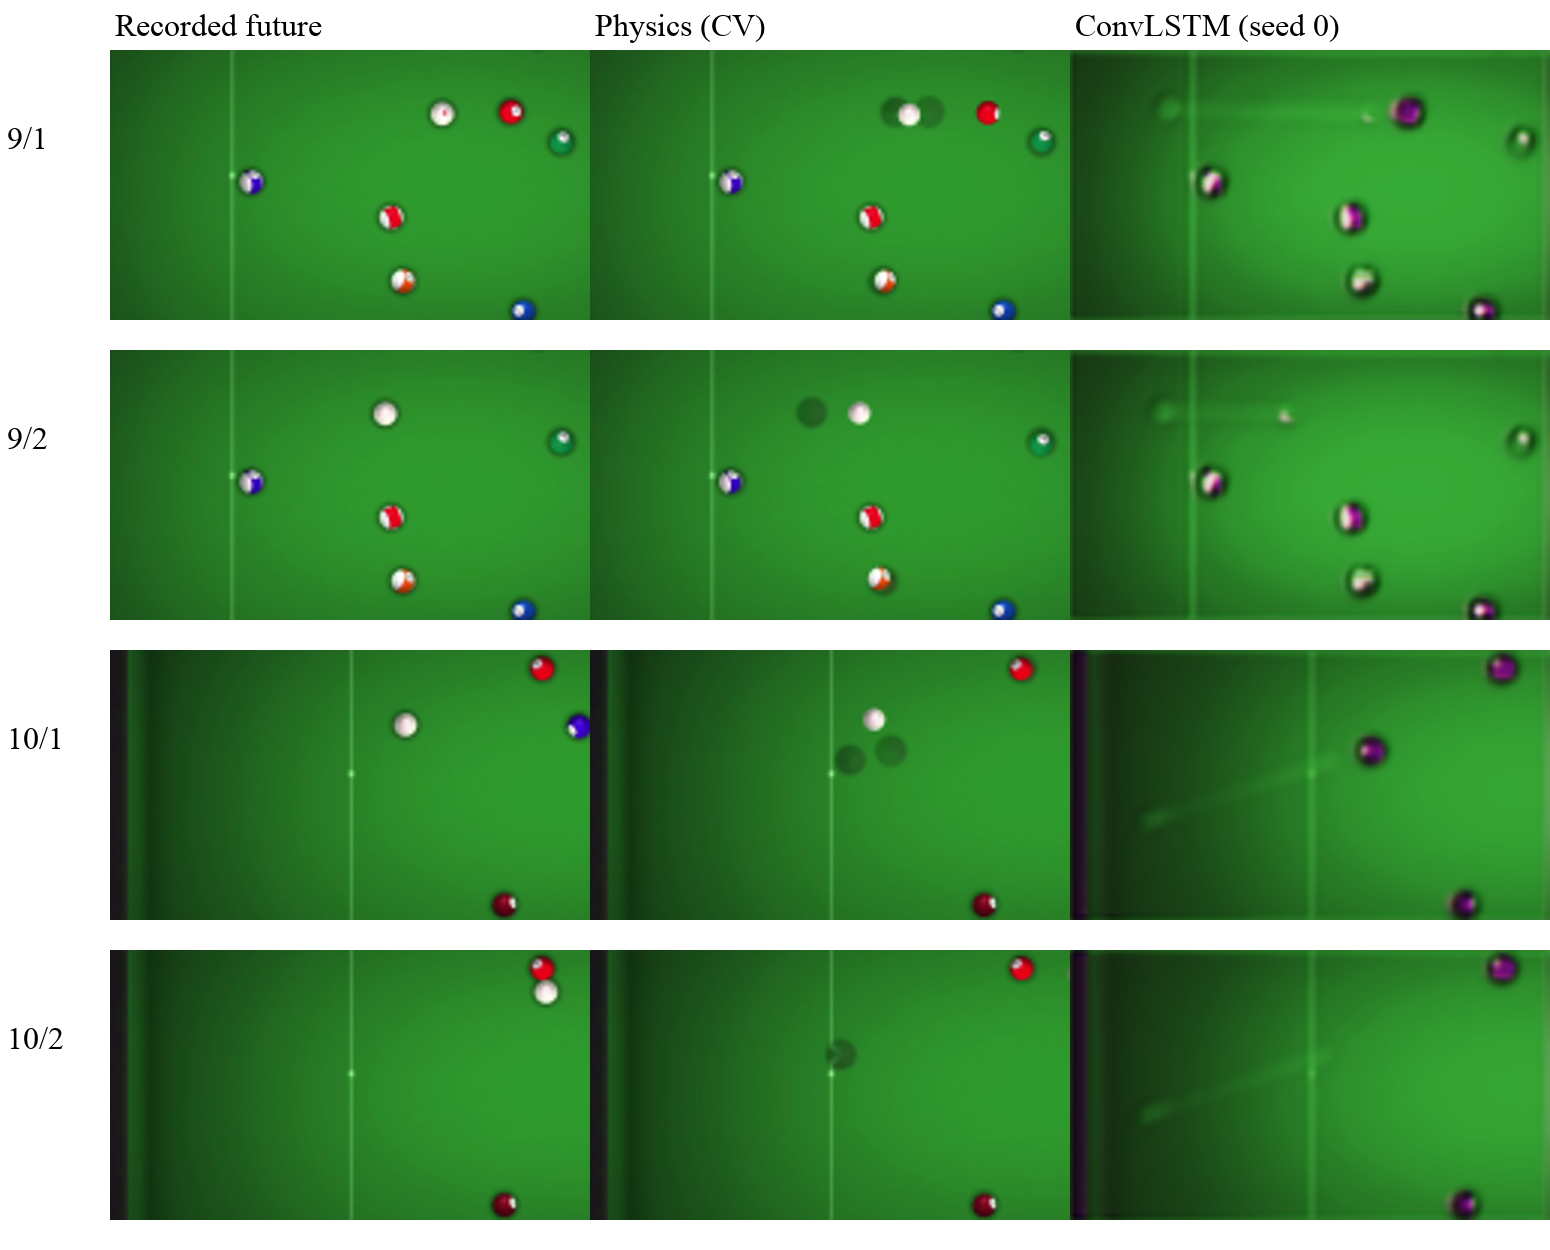
\includegraphics[width=0.96\linewidth]{figures/qualitative_predictions.png}
  \par\medskip
  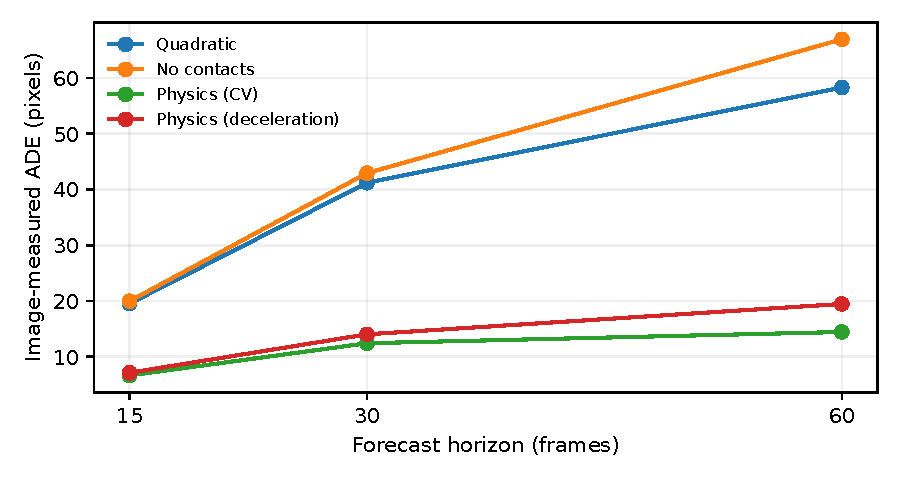
\includegraphics[width=0.78\linewidth]{figures/horizon_ade.pdf}
  \caption{Top: predictions at the thirtieth future frame for all four evaluation clips, ordered 9/1, 9/2, 10/1, and 10/2. Columns show the recorded future, constant-velocity contact simulation with the shared patch renderer, and ConvLSTM seed 0. The neural example is a fixed seed; quantitative scores include all three seeds. Bottom: image-measured displacement error across horizons. The contact-disabled curve shares the initial state and integration rule with constant-velocity contact simulation. Both panels describe the existing scene collection; image-derived measurements and two evaluation groups constrain their interpretation.}
  \label{fig:qualitative}
  \label{fig:horizon}
\end{figure}

\clearpage
\bibliographystyle{plainnat}
\bibliography{references}
\end{document}
